\documentclass[11pt,a4paper]{article}

% ---------- Packages ----------
\usepackage[utf8]{inputenc}
\usepackage[T1]{fontenc}
\usepackage[margin=1in]{geometry}
\usepackage{amsmath, amssymb}
\usepackage{graphicx}
\graphicspath{{images/}}
\usepackage{booktabs}
\usepackage{caption}
\usepackage{subcaption}
\usepackage{float}
\usepackage{hyperref}
\usepackage{cite}

% ---------- Title ----------
\title{LBD-Q-SAT: Learning SAT Branching Heuristics with Graph Neural Networks and Clause-Quality Reward Shaping}
\author{Arnab Mukhopadhyay -- arnab.mukhopadhyay@studio.unibo.it}
\date{October 2026}

\begin{document}

\maketitle

% ---------- Abstract ----------
\begin{abstract}
Modern SAT solvers use a method called CDCL (Conflict-Driven Clause Learning), which repeatedly decides which variable to assign next while searching for a solution. This decision is normally made using a fixed, hand-designed rule (e.g., VSIDS). In this project, I replaced that rule with a reinforcement learning agent: a graph neural network (GNN) that looks at the current state of the problem, represented as a variable-clause graph, and learns through trial and error which variable to branch on next in order to solve problems with fewer decisions. The agent is trained using deep Q-learning (DQN), where the GNN approximates the Q-function over possible branching decisions, and learns by directly interacting with a CDCL solver written in Python for this project. I based my approach on the Graph-Q-SAT framework, but introduced my own extension: instead of using only a flat per-decision reward as in the original work, I shaped the reward using the literal block distance (LBD) of clauses learned after each decision, a standard measure of learned-clause quality in modern SAT solvers. I compared this LBD-shaped reward against the original flat reward. Both agents need 17\% to 52\% fewer decisions than VSIDS and keep this advantage on formulas four times larger than those seen in training, and the LBD-shaped reward performs on par with the flat reward, with no significant difference on any evaluation set.
\end{abstract}

% Optional contents page (remove if not needed)
\tableofcontents
\newpage

% ====================================================
\section{Introduction}
\label{sec:intro}

SAT asks whether the variables of a Boolean formula can be set so that the whole formula is true. It is NP-complete and appears in verification, planning and scheduling. Most modern solvers, such as MiniSat~\cite{een2003minisat}, use conflict-driven clause learning (CDCL)~\cite{marques1999grasp}: the solver picks a variable, gives it a value, propagates the consequences, and learns a new clause whenever it hits a contradiction.

The choice of the next variable, the branching decision, strongly affects search time. Solvers usually rely on the hand-written VSIDS rule~\cite{moskewicz2001chaff}. Graph-Q-SAT~\cite{kurin2020gqsat} showed that this rule can be learned instead: the solver state becomes a graph, a graph neural network scores each decision, and the network is trained with deep Q-learning~\cite{mnih2015dqn} using a small penalty for every decision. That reward ignores what the solver learns along the way. The quality of learned clauses is commonly measured by the literal block distance (LBD)~\cite{audemard2009glucose}, and since the LBD of every new clause is known right after each decision, it is a natural addition to the reward.

This project, LBD-Q-SAT, introduces such a reward. Graph-Q-SAT is reimplemented from scratch, and two agents are trained that differ only in their reward: one gets the flat penalty, the other also pays for learned clauses with a high LBD. Both are compared with each other and with VSIDS, DLIS and random branching. To keep the project manageable, the agents control a small CDCL solver written in Python, without restarts or clause deletion, so results are reported in decisions rather than running time. As a warm-up, NeuroSAT~\cite{selsam2019neurosat} is also reimplemented on the same data.

Both agents solve formulas with fewer decisions than the classical rules, also on formulas four times larger than those seen in training. The LBD agent performs on par with the Graph-Q-SAT-reward agent, with no significant difference on any evaluation set, and both learn clauses of better quality than VSIDS, which makes the LBD reward a viable alternative to the flat reward. Section~\ref{sec:related} covers related work, Sections~\ref{sec:method} and~\ref{sec:experiments} the method and setup, Sections~\ref{sec:results} and~\ref{sec:discussion} the results and discussion, and Section~\ref{sec:conclusion} concludes.

% ====================================================
\section{Related Work}
\label{sec:related}

\paragraph{CDCL and branching.} A CNF formula is a set of clauses, each an OR of literals. CDCL~\cite{marques1999grasp} extends DPLL search with unit propagation and clause learning: on a conflict, the solver learns a clause that blocks the responsible assignments, usually with the first-UIP scheme, and backjumps. DLIS~\cite{marques1999branching} picks the literal occurring in the most unsatisfied clauses, while VSIDS~\cite{moskewicz2001chaff} picks the variable with the highest decaying activity score, raised whenever the variable takes part in a conflict.

\paragraph{Literal block distance.} Each decision opens a new decision level. Audemard and Simon~\cite{audemard2009glucose} defined the LBD of a learned clause as the number of distinct decision levels among its literals, and showed that low-LBD clauses are reused far more often. Their solver Glucose keeps these clauses, and clauses with an LBD of two are called glue clauses. Here LBD is used as part of a reward rather than for clause deletion.

\paragraph{Learning for SAT.} Graph neural networks suit SAT because a formula is naturally a graph of variables and clauses. NeuroSAT~\cite{selsam2019neurosat} learns to predict satisfiability from a single label per formula. Graph-Q-SAT~\cite{kurin2020gqsat}, which this project follows, models branching in MiniSat as a Markov decision process: the state is a graph of unassigned variables and unsatisfied clauses, an action is a variable and a value, and a graph network~\cite{battaglia2018relational} outputs two Q-values per variable. On small random 3-SAT formulas it needed two to three times fewer iterations than VSIDS. Adding terms to a reward is called reward shaping~\cite{ng1999shaping}; the LBD term is not potential-based, so it changes the agent's objective, and this project tests whether that objective can match the original one.

% ====================================================
\section{Methodology}
\label{sec:method}

\subsection{Problem Formulation}

Solving one formula is treated as one episode. At each step the agent looks at the current state of the solver and picks a literal among the unassigned variables. The solver sets that literal, propagates, resolves any conflicts, and stops again either when it needs a new decision or when it knows whether the formula is satisfiable. The agent then gets a reward and the next state. All rewards are negative, so the agent is trying to solve each formula as cheaply as possible.

\subsection{Data}

Formulas are generated in pairs, following the SR($n$) idea from NeuroSAT~\cite{selsam2019neurosat}. For a chosen number of variables $n$, random clauses are added one at a time until the formula becomes unsatisfiable, which is checked with MiniSat through PySAT~\cite{ignatiev2018pysat}. That formula is the unsatisfiable half of the pair. Flipping the sign of one literal in the last clause makes it satisfiable again, and gives the other half. So the two formulas differ by a single literal but have opposite answers, which stops a model from guessing the label from simple statistics such as the number of clauses.

A clause is built by drawing its length $k$, picking $k$ different variables at random, and negating each one with probability $0.5$. The length is $k = 2 + b + g$, where $b$ is $1$ with probability $0.3$ and $0$ otherwise, and $g \geq 0$ follows a geometric distribution with $P(g = j) = 0.6^{j} \cdot 0.4$.

The training set has 10\,000 pairs, with $n$ chosen uniformly between 10 and 40. The validation and test sets have 1\,000 pairs each from the same range, and three more test sets have 200 pairs each with exactly 40, 60 and 80 variables. A training formula has about 105 clauses on average.

\subsection{The Solver}

The agents control a CDCL solver written in Python for this project. It has unit propagation, first-UIP clause learning, backjumping and VSIDS with a decay factor of $0.95$. It has no restarts, no clause deletion and no phase saving, and its VSIDS rule always sets the chosen variable to false. These parts were left out to keep the code short. They are important in large solvers, but probably matter much less on formulas as small as these.

The solver is used through two calls. \texttt{start} propagates the original formula before any decision. \texttt{step} takes a literal, makes it the next decision, and keeps propagating and resolving conflicts until there is nothing left to derive or the formula is solved. One step can therefore lead to several conflicts and several learned clauses. Every time the solver learns a clause it records its LBD, and \texttt{step} returns the LBDs of all clauses learned during that step. This is all the extra information the LBD reward needs.

The branching rule is passed to the solver as a function, so the same solver runs VSIDS, DLIS, random branching and the trained agents, and all of them are compared under the same search procedure.

\subsection{State Representation}

The state is a graph with one node for each unassigned variable and one node for each original clause that is not yet satisfied. A variable is connected to every clause it appears in, and the edge has a sign: $+1$ if the variable appears as it is, $-1$ if it appears negated. Assigned variables and satisfied clauses are dropped, so the graph gets smaller as the search goes on. The nodes have no other features, so the network only sees the structure of the remaining formula.

Learned clauses are not part of the graph. This keeps the graph small and the code simple, but it means the agent does not see everything the solver knows.

\subsection{Q-Network}

The Q-network is a small graph neural network with hidden size $d = 64$. All variable nodes start from the same learned vector, and all clause nodes from another one. The network then runs $T = 4$ rounds of message passing. In each round, every clause first collects messages from its variables, and then every variable collects messages from its clauses:
\begin{align}
    m_c &= \sum_{v \in N(c)} f_{\mathrm{vc}}\big([h_v,\, \sigma_{vc}]\big), &
    h_c &\leftarrow \mathrm{LN}\big(h_c + g_{\mathrm{c}}([h_c,\, m_c])\big), \label{eq:clause_update} \\
    m_v &= \sum_{c \in N(v)} f_{\mathrm{cv}}\big([h_c,\, \sigma_{vc}]\big), &
    h_v &\leftarrow \mathrm{LN}\big(h_v + g_{\mathrm{v}}([h_v,\, m_v])\big). \label{eq:var_update}
\end{align}
Here $h_v$ and $h_c$ are the current vectors of variable $v$ and clause $c$, $N(\cdot)$ are the neighbours of a node, $\sigma_{vc}$ is the sign of the edge, $[\cdot,\cdot]$ means concatenation and LN is layer normalisation. The functions $f_{\mathrm{vc}}$, $f_{\mathrm{cv}}$, $g_{\mathrm{c}}$ and $g_{\mathrm{v}}$ are small MLPs with one hidden layer of 64 units and ReLU, and the same weights are used in every round. After the last round, one more MLP turns each variable vector into two numbers:
\begin{equation}
    \big(Q(s, \neg v),\; Q(s, v)\big) = f_{\mathrm{q}}(h_v),
    \label{eq:q_head}
\end{equation}
the value of setting $v$ to false and the value of setting it to true. A state with $k$ unassigned variables therefore has $2k$ possible actions. The network has 46\,274 parameters, and because the same weights are applied at every node, it works on formulas of any size.

\subsection{Rewards}

The flat reward, as in Graph-Q-SAT, is the same for every decision:
\begin{equation}
    r_t^{\mathrm{flat}} = -p, \qquad p = 0.1 .
    \label{eq:flat_reward}
\end{equation}
For a learned clause $c$, where $\mathrm{level}(\ell)$ is the decision level at which the variable of literal $\ell$ was assigned,
\begin{equation}
    \mathrm{lbd}(c) = \big|\{\, \mathrm{level}(\ell) : \ell \in c \,\}\big| .
    \label{eq:lbd}
\end{equation}
The LBD reward adds a cost for each clause learned during the step whose LBD is above two:
\begin{equation}
    r_t^{\mathrm{LBD}} = -p \;-\; \lambda \sum_{c \in L_t} \max\big(\mathrm{lbd}(c) - 2,\; 0\big), \qquad \lambda = 0.02 ,
    \label{eq:lbd_reward}
\end{equation}
where $L_t$ is the set of clauses learned during step $t$. Glue clauses are free. For example, a step that learns one clause with an LBD of 5 costs $0.16$ instead of $0.10$. If a step has no conflict, or only produces clauses with an LBD of one or two, both rewards are exactly the same.

\subsection{Training}

Both agents are trained with deep Q-learning~\cite{mnih2015dqn}. Each transition (state, action, reward, next state) goes into a replay buffer that holds 20\,000 of them. Once the buffer has 500 transitions, every step of the solver is followed by one update on a random batch of 32 transitions. The network is trained to bring $Q(s_t, a_t)$ close to the target
\begin{equation}
    y_t = r_t + \gamma \max_{a'} \bar{Q}(s_{t+1}, a'),
    \label{eq:target}
\end{equation}
using the Huber loss, with $\gamma = 0.99$. Here $\bar{Q}$ is a target network, a copy of the main network that is refreshed every 500 steps, and the second term is left out when the formula has been solved. The optimiser is Adam with a learning rate of $10^{-4}$, and gradients are clipped at a norm of 1. Actions are chosen $\epsilon$-greedily, with $\epsilon$ going down linearly from $1.0$ to $0.05$ over 10\,000 steps.

Each agent is trained for 1\,500 episodes, each on a random training formula. An episode is cut off after 300 decisions, and the cut-off is not treated as the end of the problem. Every 100 episodes the greedy agent is run on 100 validation formulas, and the weights with the fewest decisions on average are kept. The formulas are small, so an episode takes only a few decisions, and the whole run is only about 5\,000 steps. As a result, $\epsilon$ only gets down to about $0.53$ by the end of training.

The two agents use the same network, hyperparameters, training formulas and random seed, so they even start from the same weights. The reward is the only thing that differs.

\subsection{Differences from Graph-Q-SAT}

Table~\ref{tab:differences} lists the main differences from the original work. Most of them follow from the first one: a Python solver is far slower than MiniSat, which limits both the size of the formulas and the length of training.

\begin{table}[H]
    \centering
    \caption{Main differences between Graph-Q-SAT~\cite{kurin2020gqsat} and this project.}
    \label{tab:differences}
    \begin{tabular}{lp{0.3\linewidth}p{0.4\linewidth}}
        \toprule
        & Graph-Q-SAT & This project \\
        \midrule
        Solver & MiniSat & Python CDCL without restarts or clause deletion \\
        Network & Graph network~\cite{battaglia2018relational} & Message passing between variable and clause nodes \\
        Training formulas & Random 3-SAT & SR($n$) pairs with 10 to 20 variables \\
        Reward & Flat step penalty & Flat step penalty and LBD variant \\
        \bottomrule
    \end{tabular}
\end{table}

\subsection{Warm-up: NeuroSAT}

Before the reinforcement learning part, NeuroSAT~\cite{selsam2019neurosat} was reimplemented on the same data, as a simpler first exercise with graph neural networks for SAT. Its graph has one node per literal and one per clause. In each round, clauses add up messages from their literals, and literals add up messages from their clauses and also look at the vector of their own negation. Both updates use LSTM cells. After the last round each literal gives a vote, and the average vote decides whether the formula is predicted satisfiable. The model uses vectors of size 128 and 26 rounds, which gives 462\,209 parameters, and is trained with binary cross-entropy for 50 epochs, using Adam with a learning rate of $2 \cdot 10^{-5}$, batches of 32 formulas and gradient clipping at $0.65$. Unlike the original, the LSTM cells have no layer normalisation.

% ====================================================
\section{Experiments}
\label{sec:experiments}

\subsection{Datasets}

The reinforcement learning experiments use these subsets of the data:

\begin{itemize}
    \item \textbf{Training:} 2\,000 formulas picked at random from the 6\,972 training formulas with at most 20 variables (51\% satisfiable).
    \item \textbf{Validation:} 100 validation formulas with at most 20 variables, used only to choose the best checkpoint.
    \item \textbf{Evaluation:} 400 test formulas with 10 to 40 variables, and the first 100 formulas of the test sets with 40 and with 60 variables. The 40 and 60 sets are half satisfiable and half unsatisfiable, since they are made of pairs.
    \item \textbf{Generalization:} the first 50 formulas with 80 variables, four times the largest size seen in training.
\end{itemize}

Training and evaluation formulas come from different splits, so the agents never see an evaluation formula during training. NeuroSAT is trained on the full training set and tested on all the test sets.

\subsection{Baselines}

The three classical rules run inside the same solver as the agents. VSIDS is the solver's own rule described above. DLIS picks the literal that appears most often in the original clauses that are not yet satisfied. Random picks an unassigned variable and a value uniformly at random.

\subsection{How Hard Is the Benchmark?}

Before looking at the agents, it helps to know how hard these formulas are for the solver. This shows how much room there is for a better branching rule, and how often the LBD reward can even differ from the flat one. Table~\ref{tab:benchmark} gives the average cost with VSIDS.

\begin{table}[H]
    \centering
    \caption{Average cost of solving the formulas with VSIDS, by number of variables.}
    \label{tab:benchmark}
    \begin{tabular}{lccc}
        \toprule
        Variables & Decisions & Conflicts & Mean LBD \\
        \midrule
        10--19 & 3.22 & 2.10 & 1.04 \\
        20--29 & 5.17 & 2.42 & 1.12 \\
        30--39 & 6.60 & 2.66 & 1.21 \\
        40 & 7.82 & 3.11 & 1.31 \\
        60 & 11.55 & 4.13 & 1.71 \\
        80 & 15.86 & 4.84 & 1.69 \\
        \bottomrule
    \end{tabular}
\end{table}

These formulas are easy. Even with 80 variables the solver needs about 16 decisions and 5 conflicts, and the formulas used for training (at most 20 variables) need only about three decisions. Figure~\ref{fig:baseline_decisions} shows that the three classical rules are almost equal: on the 10--40 set they need 5.4 (VSIDS), 5.2 (DLIS) and 5.3 (random) decisions on average. With so few conflicts, VSIDS has very little information to go on and behaves much like a random choice.

\begin{figure}[H]
    \centering
    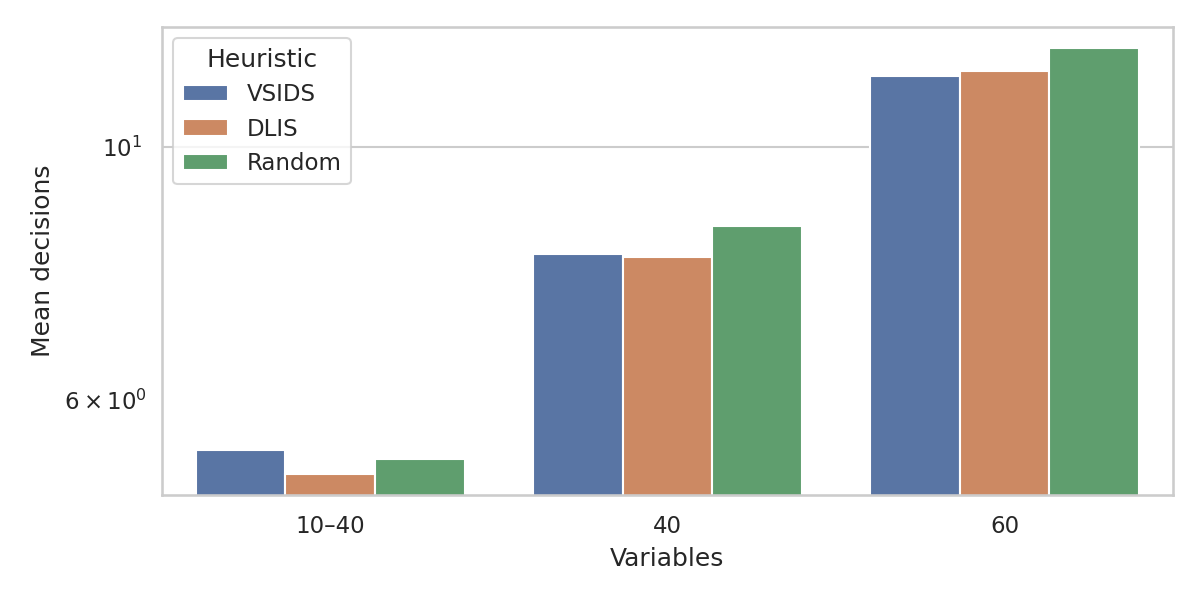
\includegraphics[width=0.8\linewidth]{baseline_decisions.png}
    \caption{Average number of decisions of the three classical rules on each evaluation set (log scale).}
    \label{fig:baseline_decisions}
\end{figure}

The learned clauses are also good from the start. Figure~\ref{fig:baseline_lbd} shows that on the 10--40 set about 62\% of learned clauses have an LBD of one and another 28\% have an LBD of two. So around 90\% are glue clauses for every rule, and none has an LBD above five. Since the LBD reward only adds a cost for an LBD of three or more, on this benchmark it differs from the flat reward on only a small share of steps. The LBD of a run is still linked to how hard it is: across formulas, the Spearman correlation between the mean LBD and the number of decisions is about $0.5$ for all three rules. Part of this is simply because harder formulas have more conflicts deeper in the search.

\begin{figure}[H]
    \centering
    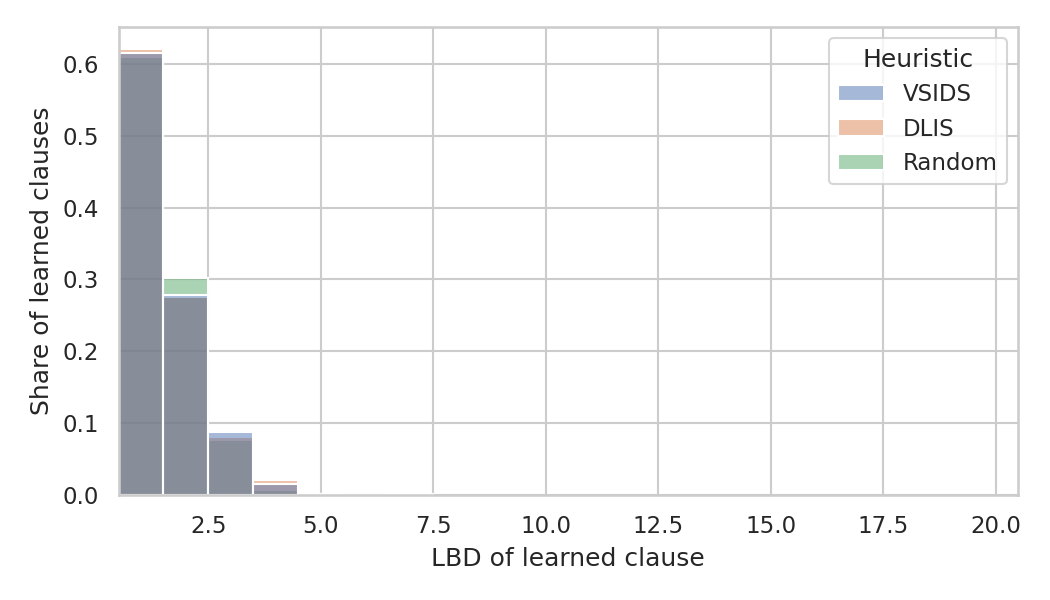
\includegraphics[width=0.8\linewidth]{baseline_lbd_distribution.png}
    \caption{LBD of the learned clauses for the three classical rules on the 10--40 set.}
    \label{fig:baseline_lbd}
\end{figure}

\subsection{Evaluation Protocol and Metrics}

Every method solves every evaluation formula once. The agents always take the action with the highest Q-value and use their best validation checkpoint. Runs are capped at 5\,000 decisions, and no run reached the cap. All methods see the same formulas, so they can be compared formula by formula. DLIS and random branching are not run on the 80-variable set.

The following measures are reported:

\begin{itemize}
    \item \textbf{Correctness:} every answer is checked against the MiniSat label, and every satisfying assignment against the formula.
    \item \textbf{Decisions:} the main measure. The median is given as well as the mean, because a few hard formulas can pull the mean up, and satisfiable and unsatisfiable formulas are also reported separately.
    \item \textbf{Clause quality:} the mean LBD of all learned clauses on a set, and the share of glue clauses (LBD of at most two).
    \item \textbf{Win rate:} on what share of formulas one method needs fewer, more or the same number of decisions as another.
    \item \textbf{Significance:} a two-sided Wilcoxon signed-rank test on the paired decision counts of the two agents. Formulas where both need the same number of decisions are left out of the test.
    \item \textbf{Time:} the average time per formula. This is only for reference, since the agents run a neural network at every decision.
\end{itemize}

For NeuroSAT, the report gives accuracy on satisfiable and unsatisfiable formulas, how accuracy changes when the network runs more rounds at test time (from 4 to 128), and how often a satisfying assignment can be read out. To read one out, the final literal vectors are split into two groups with $k$-means, and both ways of calling one group true are tried. This counts as a success only if the assignment really satisfies the formula.

\subsection{Implementation}

Everything is written in Python with PyTorch and run on Google Colab with a GPU, with the random seed 42. Training one agent takes about two minutes. One decision by the Q-network takes about 3.9\,ms, compared with 0.007\,ms for VSIDS.

% ====================================================
\section{Results}
\label{sec:results}

\subsection{Solver Correctness}

The Python solver gives the same answer as MiniSat on every formula it was checked on: 500 test formulas solved once with VSIDS and once with random branching, and 300 formulas with 40, 60 and 80 variables. Every satisfying assignment it returned was valid. In the main evaluation, all 3\,150 runs (five methods on 600 formulas, and three methods on the 50 formulas with 80 variables) finished with the correct answer. The decision counts below therefore compare methods that all solve the formulas correctly.

\subsection{Training}

Figure~\ref{fig:dqn_validation} shows the mean number of decisions on the validation formulas during training. Both agents first get worse: around episode 300 they need more than 6 decisions, almost twice as many as random branching (3.5). At this point $\epsilon$ is still about $0.9$, the replay buffer is filled with nearly random actions, and the network has not yet learned anything useful. Between episodes 700 and 800 both agents improve sharply, and from then on they stay at about 2.3 decisions, below VSIDS (3.2) and random branching. The best checkpoint of each agent needs 2.2 decisions on average. Each run took 1.8 to 1.9 minutes.

\begin{figure}[H]
    \centering
    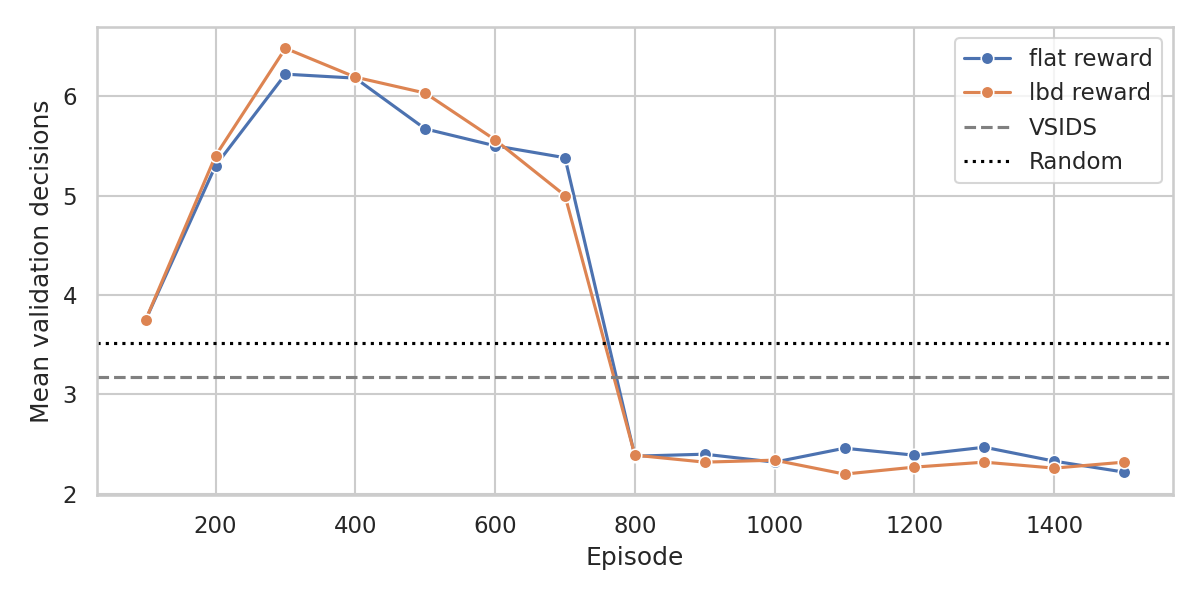
\includegraphics[width=0.75\linewidth]{dqn_validation.png}
    \caption{Mean number of decisions on the 100 validation formulas during training, for both rewards. The dashed and dotted lines show VSIDS and random branching.}
    \label{fig:dqn_validation}
\end{figure}

The two curves are almost the same. At episode 100 both agents need exactly 3.8 decisions, and both runs had taken exactly 384 steps by then, which suggests that the two agents had behaved the same way so far. Since they start from the same weights and see the same formulas, the runs only drift apart on steps where the solver learns a clause with an LBD above two. From episode 800 onwards both agents stay well below VSIDS and random branching and end at the same best value of 2.2 decisions.

\subsection{Agents Against the Classical Rules}

Table~\ref{tab:median_decisions} and Figure~\ref{fig:final_decisions} give the median number of decisions on each evaluation set.

\begin{table}[H]
    \centering
    \caption{Median number of decisions per formula (lower is better). The last two columns give the median of each agent divided by the median of VSIDS.}
    \label{tab:median_decisions}
    \small
    \begin{tabular}{lccccccc}
        \toprule
        Variables & VSIDS & DLIS & Random & Q flat & Q LBD & Q flat / VSIDS & Q LBD / VSIDS \\
        \midrule
        10--40 & 4.0 & 4.0 & 4.0 & 3.0 & 3.0 & 0.75 & 0.75 \\
        40 & 6.0 & 6.5 & 8.0 & 5.0 & 5.0 & 0.83 & 0.83 \\
        60 & 11.5 & 10.5 & 11.0 & 5.5 & 6.0 & 0.48 & 0.52 \\
        80 & 14.0 & -- & -- & 9.0 & 8.0 & 0.64 & 0.57 \\
        \bottomrule
    \end{tabular}
\end{table}

\begin{figure}[H]
    \centering
    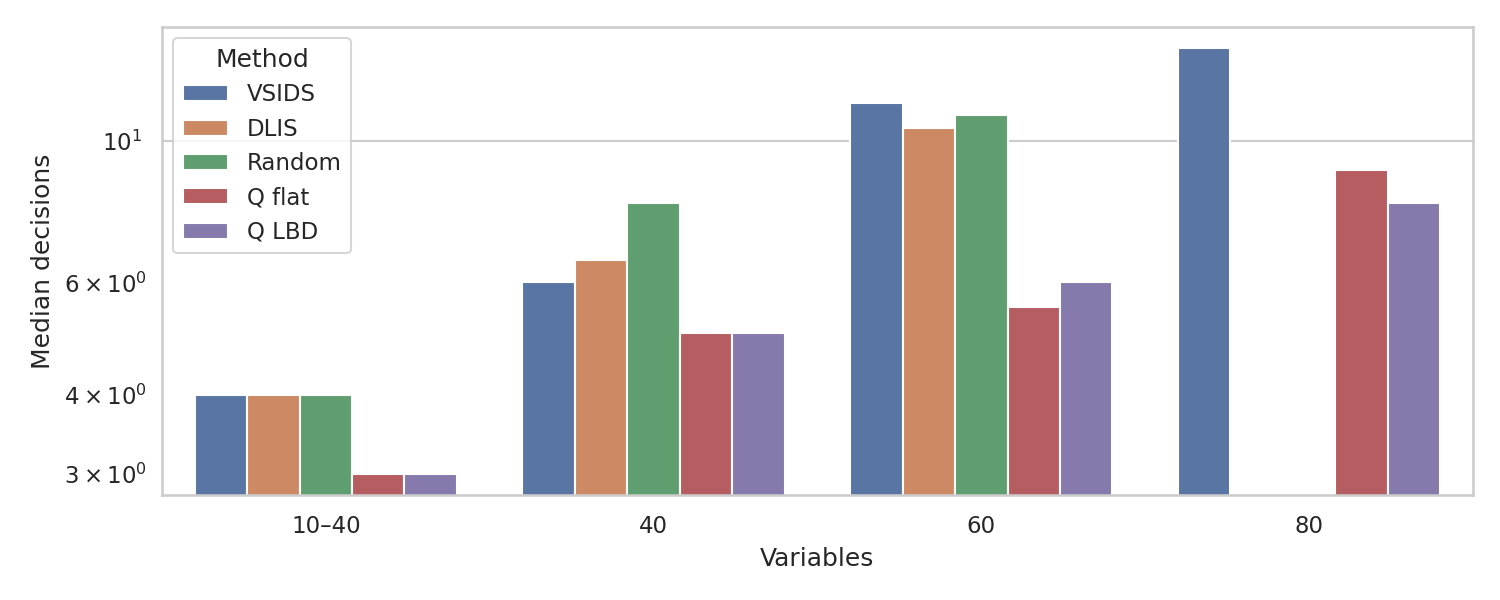
\includegraphics[width=0.85\linewidth]{final_decisions.png}
    \caption{Median number of decisions for every method on each evaluation set (log scale). DLIS and random branching were not run on the 80-variable set.}
    \label{fig:final_decisions}
\end{figure}

Both agents beat all three classical rules on every set. They need between 48\% and 83\% of the decisions VSIDS needs, and the gap grows with the size of the formulas. The means tell the same story: on the 60-variable set VSIDS needs 11.6 decisions on average and the two agents 6.8 and 7.1. The agents keep their advantage on the 80-variable formulas, which are four times larger than anything they saw during training. This works because the network uses the same weights at every node, so nothing in it depends on the number of variables.

Counted formula by formula, the LBD agent needs fewer decisions than VSIDS on 61\% of the 10--40 formulas and more on 16\%. On the larger sets the gap is wider: it wins on 66\%, 82\% and 84\% of the formulas with 40, 60 and 80 variables, and loses on only 9\% to 12\%.

Table~\ref{tab:sat_unsat} splits the results by answer. The agents gain the most on unsatisfiable formulas. On the 10--40 set the median agent run proves unsatisfiability after a single decision, against three for VSIDS, and on the 80-variable set it needs 2 decisions against 8. The SR($n$) construction explains why this is possible: an unsatisfiable formula becomes unsatisfiable only through its last clause, so a small group of clauses is enough to show the contradiction. An agent that learns to branch into that group finds the conflict right away. On satisfiable formulas the gains are smaller but still clear, for example 14 decisions against 19 on the 80-variable set.

\begin{table}[H]
    \centering
    \caption{Median number of decisions on unsatisfiable (UNSAT) and satisfiable (SAT) formulas.}
    \label{tab:sat_unsat}
    \begin{tabular}{llccccc}
        \toprule
        Variables & Answer & VSIDS & DLIS & Random & Q flat & Q LBD \\
        \midrule
        10--40 & UNSAT & 3.0 & 2.0 & 3.0 & 1.0 & 1.0 \\
               & SAT   & 6.0 & 7.0 & 6.0 & 5.0 & 5.0 \\
        40     & UNSAT & 4.0 & 3.0 & 4.5 & 2.0 & 2.0 \\
               & SAT   & 10.0 & 11.5 & 10.5 & 7.5 & 8.0 \\
        60     & UNSAT & 5.0 & 4.5 & 5.5 & 3.0 & 3.0 \\
               & SAT   & 15.5 & 17.0 & 17.0 & 10.5 & 11.0 \\
        80     & UNSAT & 8.0 & -- & -- & 2.0 & 2.0 \\
               & SAT   & 19.0 & -- & -- & 14.0 & 14.0 \\
        \bottomrule
    \end{tabular}
\end{table}

The picture is very different for running time. The agents call the network at every decision, so a formula on the 60-variable set takes about 30 to 35\,ms with an agent and 5.4\,ms with VSIDS. Fewer decisions do not make up for the cost of the network at this scale.

\subsection{Flat Reward Against LBD Reward}

This is the main question of the project. Table~\ref{tab:flat_vs_lbd} compares the two agents formula by formula, and Figure~\ref{fig:flat_vs_lbd} plots the number of decisions of one agent against the other.

\begin{table}[H]
    \centering
    \caption{Formula-by-formula comparison of the LBD agent with the flat agent. ``Better'' means the LBD agent needs fewer decisions. The p-value is from a two-sided Wilcoxon signed-rank test.}
    \label{tab:flat_vs_lbd}
    \begin{tabular}{lcccc}
        \toprule
        Variables & Better & Worse & Tie & p-value \\
        \midrule
        10--40 & 23\% & 24\% & 53\% & 0.40 \\
        40 & 34\% & 27\% & 39\% & 0.30 \\
        60 & 34\% & 36\% & 30\% & 0.51 \\
        80 & 34\% & 38\% & 28\% & 0.38 \\
        \bottomrule
    \end{tabular}
\end{table}

\begin{figure}[H]
    \centering
    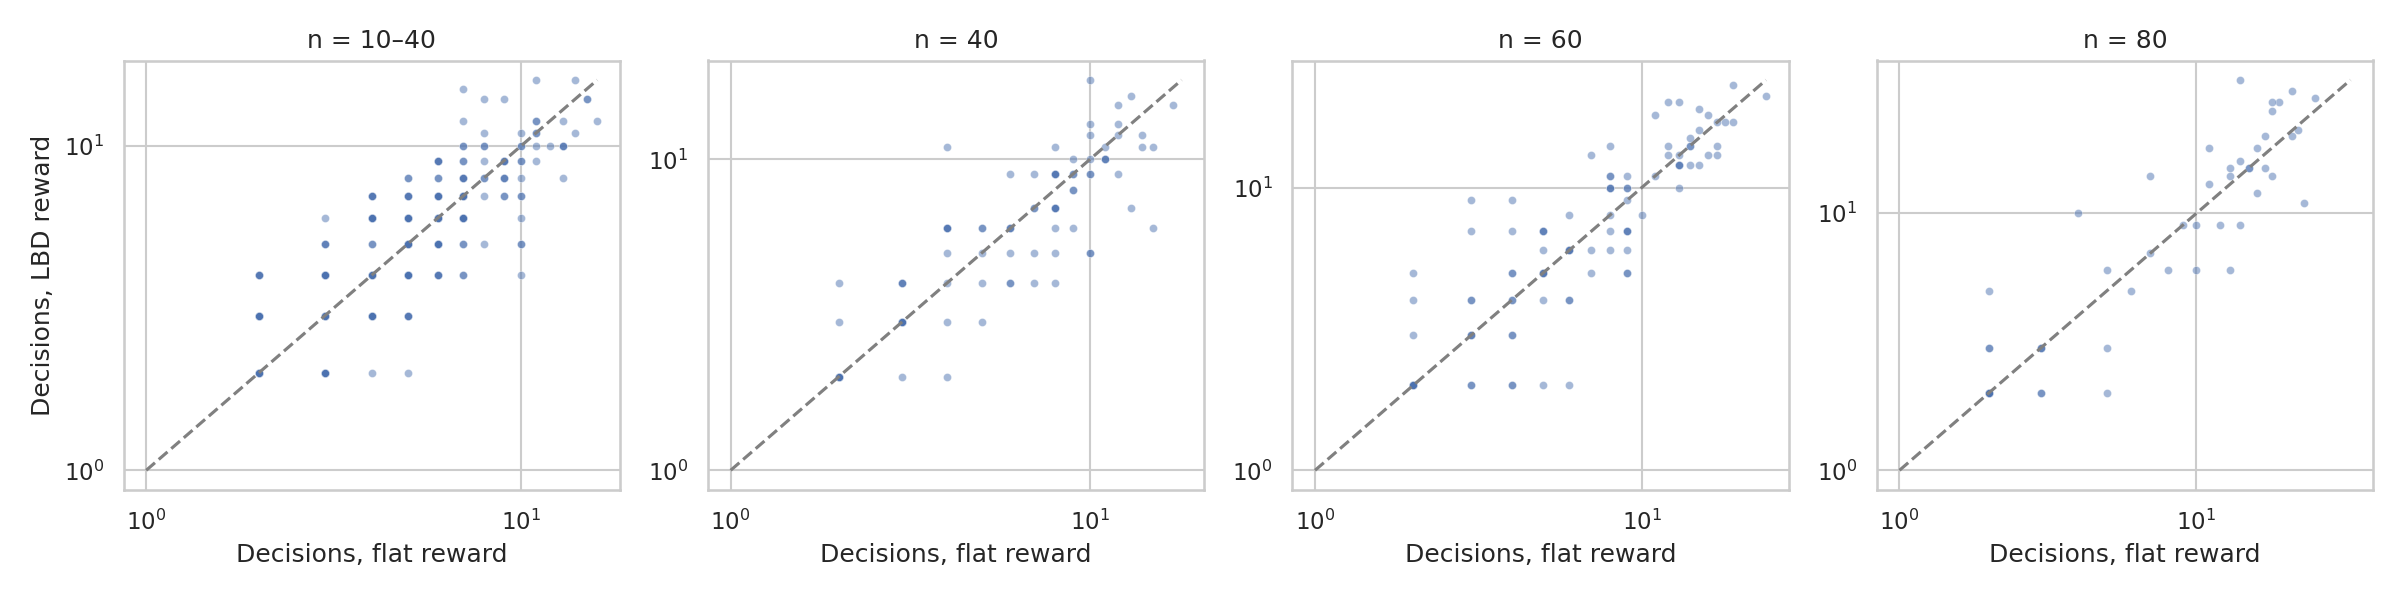
\includegraphics[width=\linewidth]{final_flat_vs_lbd.png}
    \caption{Decisions needed by the LBD agent against the flat agent, one point per formula (log scale). Points below the dashed line are formulas where the LBD agent needs fewer decisions.}
    \label{fig:flat_vs_lbd}
\end{figure}

The two agents perform on par. On every set, the LBD agent wins on about as many formulas as it loses, and the Wilcoxon test finds no significant difference on any set. In Figure~\ref{fig:flat_vs_lbd} the points are spread evenly on both sides of the diagonal. The medians in Table~\ref{tab:median_decisions} differ by at most one decision, in either direction.

\subsection{Learned Clause Quality}

The LBD reward was meant to push the solver towards learning better clauses, so it is worth checking whether it did. Table~\ref{tab:quality} reports the mean LBD and the share of glue clauses, and Figure~\ref{fig:final_lbd} shows the full distributions.

\begin{table}[H]
    \centering
    \caption{Number of learned clauses, mean LBD and share of glue clauses (LBD of at most two) over all formulas of each set.}
    \label{tab:quality}
    \small
    \begin{tabular}{lccccccccc}
        \toprule
        & \multicolumn{3}{c}{VSIDS} & \multicolumn{3}{c}{Q flat} & \multicolumn{3}{c}{Q LBD} \\
        \cmidrule(lr){2-4} \cmidrule(lr){5-7} \cmidrule(lr){8-10}
        Variables & Clauses & LBD & Glue & Clauses & LBD & Glue & Clauses & LBD & Glue \\
        \midrule
        10--40 & 811 & 1.51 & 89\% & 620 & 1.33 & 96\% & 610 & 1.34 & 96\% \\
        40 & 274 & 1.75 & 83\% & 206 & 1.51 & 88\% & 199 & 1.35 & 94\% \\
        60 & 363 & 1.95 & 76\% & 228 & 1.48 & 92\% & 252 & 1.60 & 89\% \\
        80 & 201 & 2.02 & 74\% & 117 & 1.50 & 95\% & 129 & 1.64 & 86\% \\
        \bottomrule
    \end{tabular}
\end{table}

\begin{figure}[H]
    \centering
    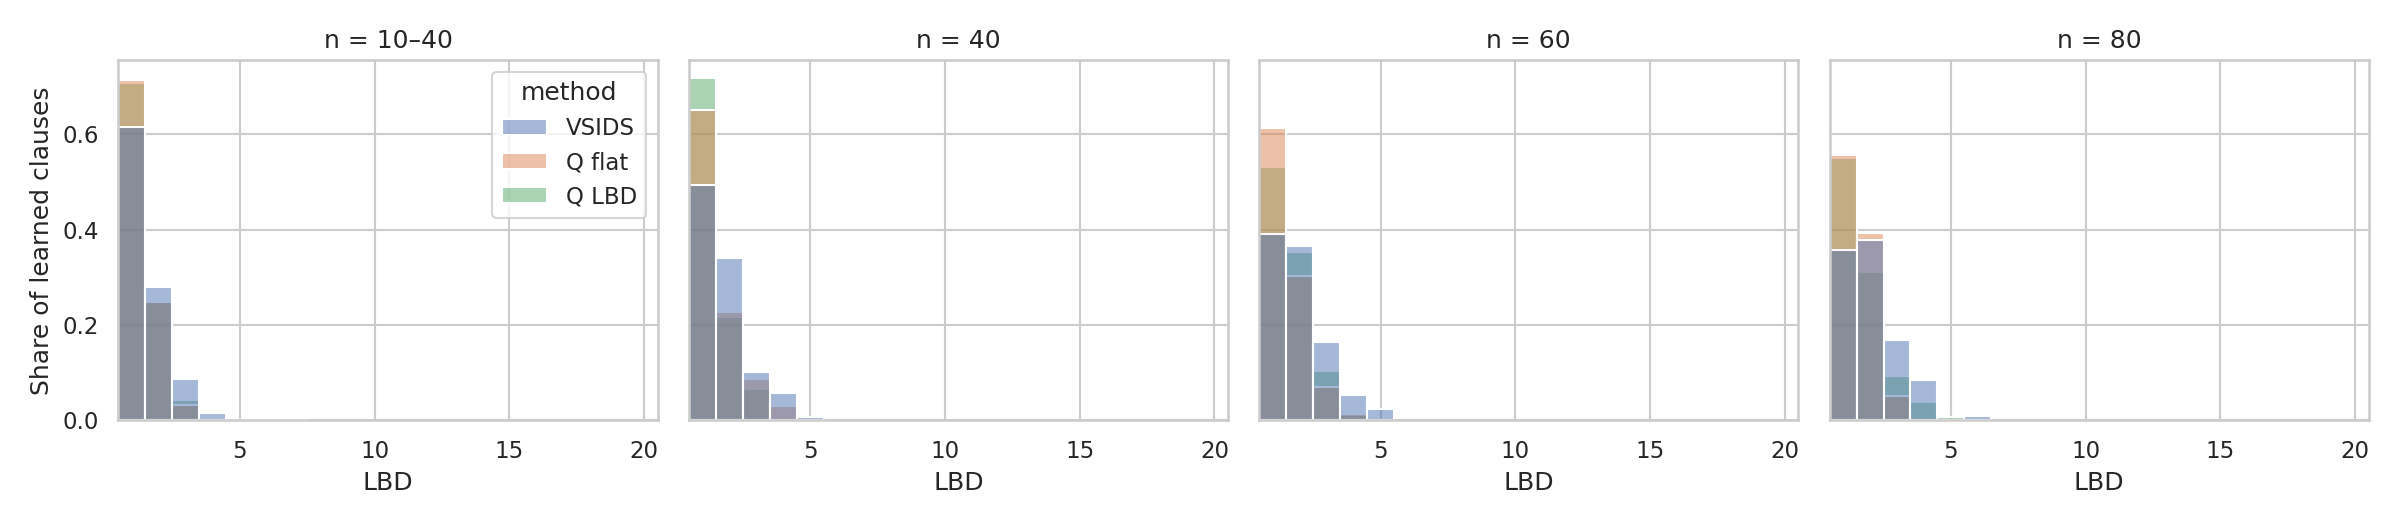
\includegraphics[width=\linewidth]{final_lbd_distribution.png}
    \caption{Distribution of the LBD of learned clauses for VSIDS and both agents on each evaluation set.}
    \label{fig:final_lbd}
\end{figure}

Both agents learn fewer clauses than VSIDS, and their clauses have a lower LBD. The difference grows with formula size: on the 80-variable set the mean LBD is 2.02 for VSIDS and about 1.5 to 1.6 for the agents. Between the two agents the picture depends on the set. The LBD agent learns the best clauses of all methods on the 40-variable set (mean LBD 1.35, 94\% glue clauses), the two agents are equal on the 10--40 set, and the flat agent has the lower LBD on the 60- and 80-variable sets.

\subsection{Warm-up: NeuroSAT}

NeuroSAT reaches 92.9\% accuracy on the test set with 26 rounds, the number used in training. It is better on unsatisfiable formulas (98.0\%) than on satisfiable ones (87.9\%). Training was not smooth: for the first 23 epochs the model stayed at 50\% accuracy, the level of random guessing, and then within a few epochs it jumped to above 80\%. The best validation accuracy, 94.4\%, was reached at epoch 48.

\begin{table}[H]
    \centering
    \caption{NeuroSAT accuracy and share of satisfiable formulas for which a satisfying assignment could be decoded.}
    \label{tab:neurosat}
    \begin{tabular}{lcccc}
        \toprule
        & \multicolumn{2}{c}{Accuracy} & \multicolumn{2}{c}{Assignments decoded} \\
        \cmidrule(lr){2-3} \cmidrule(lr){4-5}
        Variables & 26 rounds & Best & 26 rounds & 128 rounds \\
        \midrule
        10--40 & 92.9\% & 97.6\% & 86.8\% & 96.8\% \\
        40 & 88.0\% & 96.3\% & 80.5\% & 96.5\% \\
        60 & 82.5\% & 93.0\% & 64.0\% & 88.5\% \\
        80 & 69.5\% & 86.8\% & 51.5\% & 76.5\% \\
        \bottomrule
    \end{tabular}
\end{table}

Table~\ref{tab:neurosat} and Figure~\ref{fig:neurosat_rounds} show what happens when the model runs for more rounds than it was trained with. Accuracy keeps rising well past 26 rounds, and the larger the formulas, the more the extra rounds help. On the 80-variable set, accuracy goes from 69.5\% at 26 rounds to 86.8\% at 128 rounds. For most satisfiable formulas a valid assignment can be read out of the literal vectors, up to 96.8\% on the 10--40 set with 128 rounds. These results agree with what the original paper reports: the network seems to carry out an iterative search, and larger formulas need more iterations.

\begin{figure}[H]
    \centering
    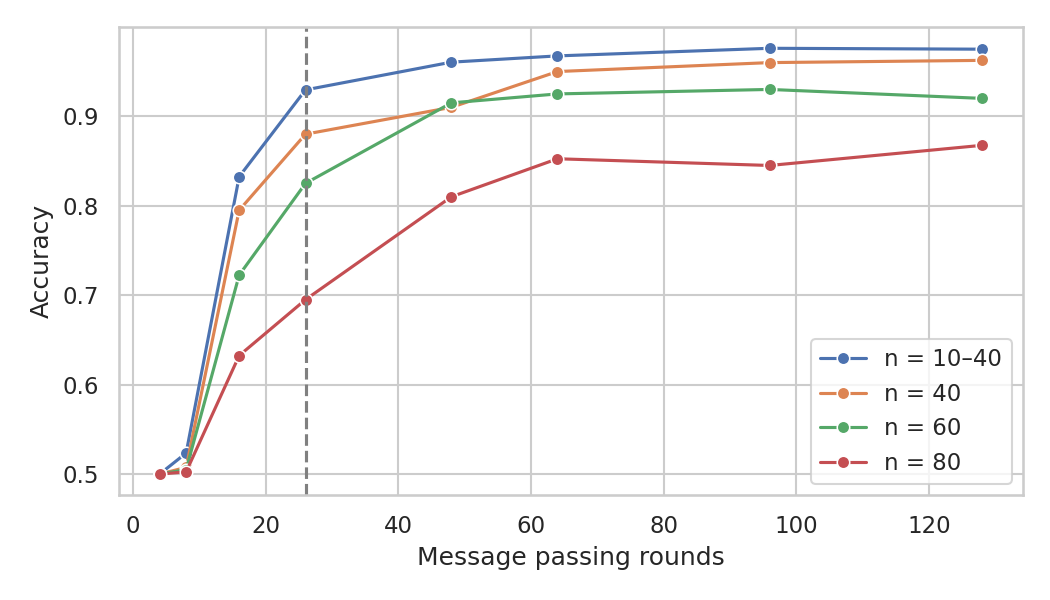
\includegraphics[width=0.7\linewidth]{accuracy_vs_rounds.png}
    \caption{NeuroSAT accuracy against the number of message-passing rounds at test time. The dashed line marks the 26 rounds used in training.}
    \label{fig:neurosat_rounds}
\end{figure}

% ====================================================
\section{Discussion}
\label{sec:discussion}

\subsection{A Learned Branching Policy That Beats the Classical Rules}

Both agents learned a useful branching policy. After a short training run of about 5\,000 steps, they need fewer decisions than VSIDS, DLIS and random branching on every evaluation set, and the gap is largest on the larger formulas: on the 60-variable set the agents need about half the decisions of VSIDS, and on the 80-variable set 57\% to 64\% of them. They also keep this advantage on formulas four times larger than any seen in training, because the network applies the same weights at every node and does not depend on the number of variables. This confirms the main claim of Graph-Q-SAT in a different solver and on a different family of formulas.

The largest gains are on unsatisfiable formulas, where the median agent run needs one to three decisions against three to eight for VSIDS. In SR($n$) formulas the contradiction comes from a small group of clauses, and the agents learn to branch into that group early, so the solver reaches the decisive conflict almost at once. On satisfiable formulas the gains are smaller but consistent across every set.

\subsection{The LBD Reward Matches the Graph-Q-SAT Reward}

The main contribution of this project is a new reward for learned branching, one that also takes into account the quality of the clauses the solver learns. The question for any new reward is whether an agent trained with it is at least as good as one trained with the established reward. The results show that it is. The LBD agent and the flat Graph-Q-SAT agent reach the same validation performance during training (Figure~\ref{fig:dqn_validation}), have the same median number of decisions on the 10--40 and 40-variable sets, and stay within one decision of each other on the larger sets, in median as well as in mean. On the 80-variable set, the hardest one and the furthest from the training distribution, the LBD agent has the lower median (8 decisions against 9) and the flat agent the lower mean (9.1 against 9.9). Formula by formula, neither agent is consistently ahead, and the Wilcoxon test finds no significant difference on any set (Table~\ref{tab:flat_vs_lbd}).

The LBD reward therefore gives the agent a richer training signal without any measurable loss in solving performance. It costs nothing extra to compute, since the solver already knows the LBD of every clause it learns, and it fits into the existing deep Q-learning setup without any other change. The same holds for generalisation: the LBD agent transfers to 40-, 60- and 80-variable formulas as well as the flat agent.

\subsection{Clause Quality}

Both agents learn fewer and better clauses than VSIDS (Table~\ref{tab:quality}). On the 80-variable set the mean LBD drops from 2.02 for VSIDS to 1.50 and 1.64 for the two agents, and the share of glue clauses rises from 74\% to 95\% and 86\%. The LBD agent gives the best clause quality of all methods on the 40-variable set, with a mean LBD of 1.35 and 94\% glue clauses, against 1.51 and 88\% for the flat agent and 1.75 and 83\% for VSIDS, while on the 60- and 80-variable sets the flat agent has the lower LBD. These results show that a learned branching policy steers the solver towards the kind of clauses that modern solvers such as Glucose try to keep, and that the LBD reward keeps this benefit while making clause quality an explicit part of the training objective.

\subsection{NeuroSAT}

The NeuroSAT warm-up reproduces the main behaviour reported in the original paper on a much smaller budget. It reaches 92.9\% test accuracy, and its accuracy keeps rising when it runs more message-passing rounds than it was trained with, especially on larger formulas. The long plateau at 50\% before the sudden jump in accuracy shows how hard it is to learn from one bit of supervision per formula. In an earlier run with a higher learning rate ($10^{-4}$) and 30 epochs, the model never left this plateau. Lowering the learning rate to $2 \cdot 10^{-5}$ and training for 50 epochs was enough to get past it.

% ====================================================
\section{Conclusion}
\label{sec:conclusion}

This project introduced LBD-Q-SAT, a reward for learned SAT branching that adds a clause-quality term based on the literal block distance to the flat per-decision penalty of Graph-Q-SAT. Graph-Q-SAT was reimplemented from scratch with a Python CDCL solver, and two agents differing only in their reward were compared with each other and with VSIDS, DLIS and random branching.

Both agents need 17\% to 52\% fewer decisions than VSIDS and keep this advantage on formulas four times larger than those seen in training. The main finding is that the LBD agent performs on par with the Graph-Q-SAT-reward agent under identical conditions, with no significant difference on any evaluation set, equal generalisation and better clause quality than VSIDS. As a first experiment, the aim was not to exceed Graph-Q-SAT but to match it, and this was achieved. Since it reaches the same performance while also encoding clause quality, the LBD reward is a viable alternative to the flat reward for future learned branching heuristics. The NeuroSAT warm-up reached 92.9\% test accuracy.

% ====================================================
\section*{Future Work}

\begin{itemize}
    \item \textbf{Harder benchmarks.} Larger random and structured industrial formulas, where learned clauses span many decision levels, give the LBD term more to act on.
    \item \textbf{Longer training and several seeds,} so that $\epsilon$ reaches its final value and the rewards can be compared more precisely.
    \item \textbf{Reward and state design.} Tuning $\lambda$ and the LBD threshold, rewarding glue clauses, and adding learned clauses with their LBD to the state graph.
    \item \textbf{Integration with MiniSat or Glucose,} to compare running time and let the reward interact with LBD-based clause deletion.
\end{itemize}

\section*{Acknowledgements and Academic Integrity}

Claude was used to summarise and simplify research papers, as a teaching assistant for difficult concepts behind the graph Q-network of Graph-Q-SAT, and to fix grammatical issues in this report. The idea, its formulation, all code and all experimental results in this report are the author's own work.

% ====================================================
\bibliographystyle{unsrt}
\bibliography{references}

\end{document}